\documentclass{gatech-thesis}
\usepackage{cite}
\usepackage{graphicx}


%%
%% This example is adapted from ucthesis.tex, a part of the
%% UCTHESIS class package...
%%
\title{Search for Neutrino Transients Using IceCube and DeepCore}
\author{Jacob D. Daughhetee}
\principaladviser{Professor Ignacio Taboada}
\committeechair{Professor Pablo Laguna}
\firstreader{Professor Nepomuk Otte}
\secondreader{Professor Carol Paty\\(Earth and Atmospheric Science)}
\thirdreader{Professor }
\fourthreader{Professor }
\department{School of Physics}
\degree{Doctor of Philosophy}
\copyrightyear{2014}
\submitdate{August 2014}
\bibfiles{example-thesis}
%% The following are the defaults
%%    \titlepagetrue
%%    \signaturepagetrue
%%    \copyrightfalse
%%    \figurespagetrue
%%    \tablespagetrue
%%    \contentspagetrue
%%    \dedicationheadingfalse
\bibpagetrue
%%    \thesisproposalfalse
%%    \strictmarginstrue
\begin{document}
\bibliographystyle{gatech-thesis}
%%
\begin{preliminary}
\begin{dedication}
\null\vfil
{\large
\begin{center}

\end{center}}
\vfil\null
\end{dedication}
\begin{preface}
This dissertation is based on data acquired with the IceCube Neutrino Observatory whose maintenance and operation is the result of an immense international collaborative effort. While ... (acknowledge previous work?)
\end{preface}
\begin{acknowledgements}
I want to thank my fellow graduate student office mates whose constant distractions helped me retain my sanity.
\end{acknowledgements}
% print table of contents, figures and tables here.
\contents
% if you need a "List of Symbols or Abbreviations" look into
% gatech-thesis-gloss.sty.

\begin{summary}
Observations indicate that there is a correlation between long duration gamma-ray bursts (GRBs) and core-collapse supernovae (SNe).  The leading model for GRB production assumes that relativistic jets are generated by the core-collapse within the progenitor star.  Charged particles undergo Fermi-acceleration within internal shocks of these jets and subsequently give rise to gamma ray emission once the jets breach the surrounding stellar envelope.  Very few SNe result in the occurrence of GRBs, however,  but it has been suggested that a significant fraction of core-collapse SNe manage to produce mildly relativistic jets.  These jets are insufficiently energetic to break through the envelope and are effectively 'choked' resulting in a lack of observed gamma ray emission.  In both the failed and successful GRB scenario, neutrino production can occur if protons are accelerated in the internal shocks of these jets.  These neutrinos may be detectable by the IceCube neutrino observatory and its low energy extension DeepCore.  A dedicated search for temporal and spatial clustering of neutrino events during the 2012 data season aims to reveal the presence of any 'choked' GRB events within 20 Mpc.
\end{summary}

\end{preliminary}
%%
\chapter{Introduction}

%% Neutrino Astronomy
%% Why neutrinos
%% How neutrinos (production, detection)
%% SN1987A
%% GRBs, SN, Chk GRBs

%%
\chapter{Detector}
The IceCube Neutrino Observatory is located at the geographical South Pole deep within the glacial ice of the Antarctic ice sheet. This site allowed for the use of the Amundsen-Scott South Pole station as a staging ground and logistics hub for the construction and continued operation of the detector. 

%% Insert Detector Image!

\begin{figure}
  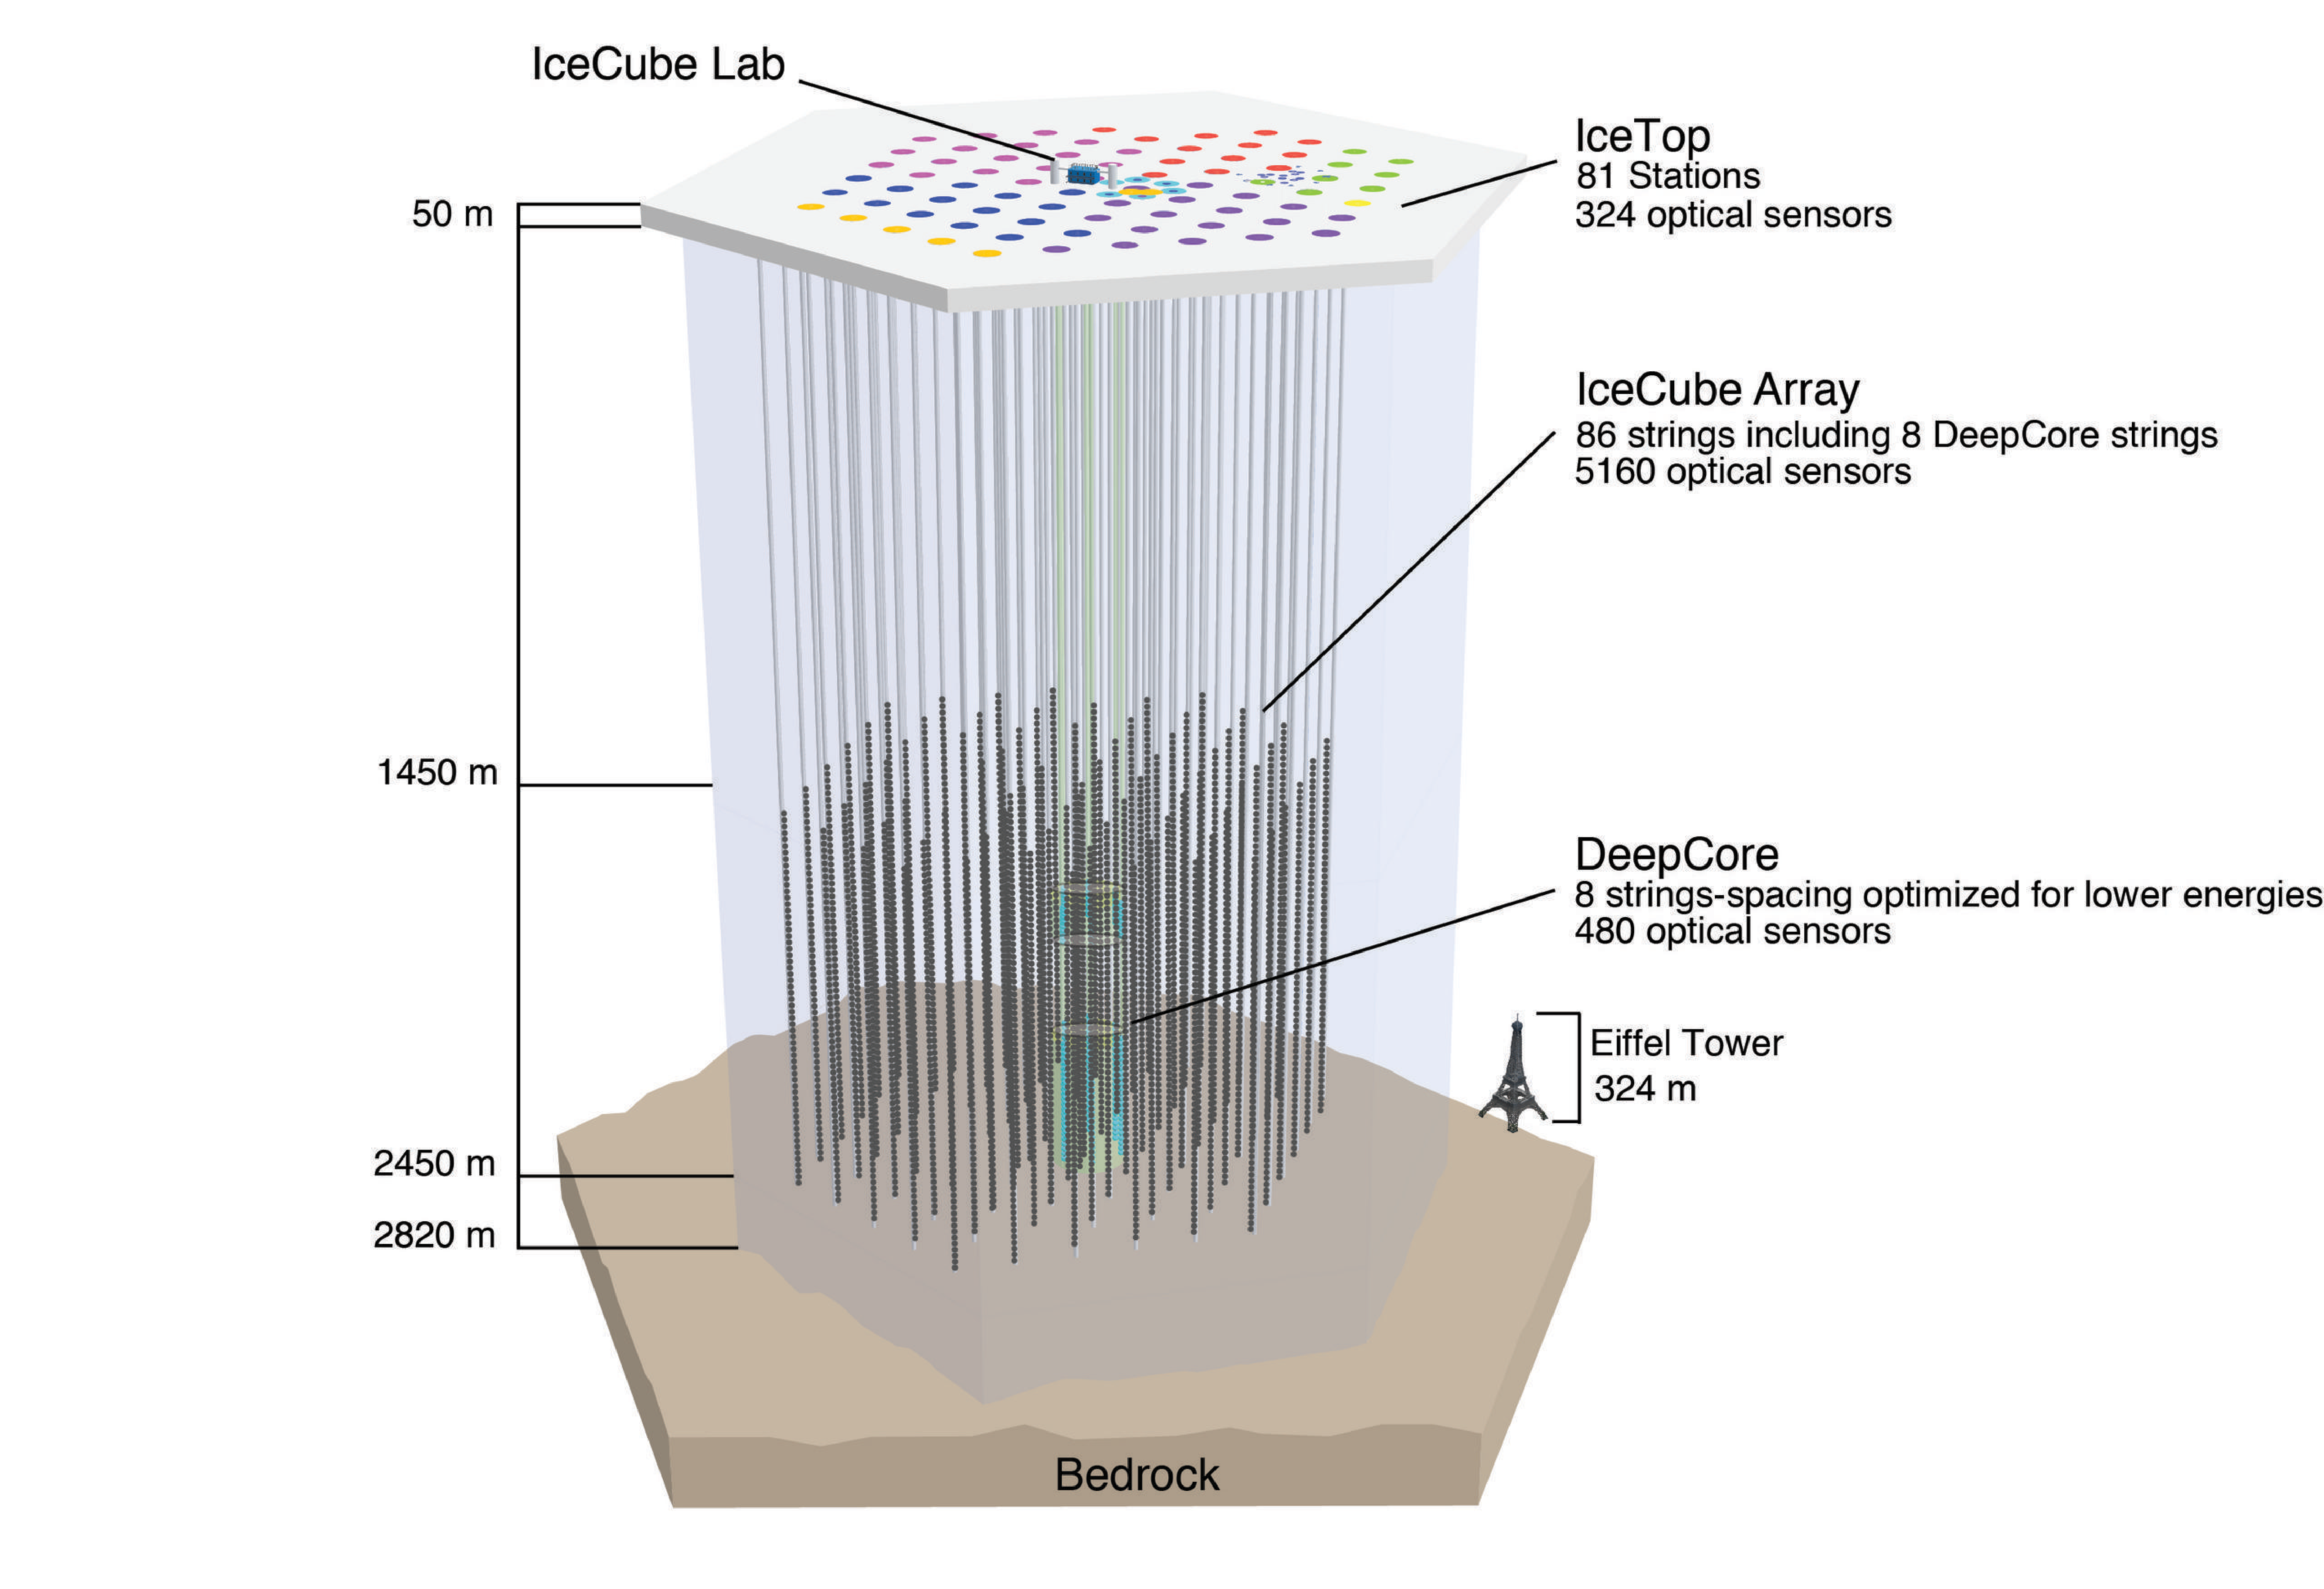
\includegraphics[width=8.5in]{ArrayWSeasonsLabels.pdf} 
\end{figure}

%% Refs: Performance of DeepCore, IceCube construction paper?

\chapter{Previous Point Source Searches}

\chapter{Data Acquisition}

\chapter{Event Selection}

\chapter{Analysis Method}

\chapter{Results}
Some other research was once performed ~\cite{Nobody06}.

\begin{figure}
\caption{A first figure.}
\end{figure}

\begin{figure}
\caption{A second figure.}
\end{figure}
%%
\chapter{Conclusion}

%% We need this since this file doesn't ACTUALLY \cite anything...
%%

\appendix
\chapter{Some Ancillary Stuff}

Ancillary material should be put in appendices, which 
appear just before the bibliography. 

\begin{postliminary}
\bibliography{jdthesis}{}

\postfacesection{Index}{%
%%             ... generate an index here
%%         look into gatech-thesis-index.sty
}
\begin{vita}

\end{vita}
\end{postliminary}
\end{document}
